\documentclass[20pt,a4paper,ngerman]{scrbook}
\usepackage{caption}
\usepackage{graphicx}
\usepackage{standalone}
\usepackage[utf8]{inputenc}
\usepackage{tabularx}
\usepackage{tikz}
\usepackage{pdfpages}
\usetikzlibrary{shapes,snakes}
\usepackage{forloop}
\usepackage{intcalc}

\usepackage{german}
\usepackage{geometry}
\geometry{
 a4paper,
 total={210mm,297mm},
 left=20mm,
 right=20mm,
 top=16mm,
 bottom=16mm,
 }
\pagenumbering{gobble}
\pagestyle{empty}
\usepackage{pgfpages} 
%\pgfpagesuselayout{2 on 1}[a4paper,border shrink=1mm,landscape]


\begin{document}

	\newcounter{stno} 
	\newcounter{groupno}
	\forloop{stno}{1}{\value{stno} < 201}
	{
	  	\setcounter{groupno}{\intcalcMod{\arabic{stno}}{4}}
	  	\stepcounter{groupno}
		\noindent
		\begin{description}
			\item[Group number/name: \thestno ] \dotfill \\
			\item[Time:] 11:00 - 14:00; 14:30 Award Ceremony
			\item[Manual:] Note down your group members below (at least 5 people) and give your group a fancy name (the best will be awarded - be creative!). After the rallye you have to hand in this sheet at the information desk. You can visit 21 stations in total to earn points. Have fun!
			\item[Participants:] \hfill \\
				\begin{enumerate}
				%	\itemsep6pt
					\item \dotfill
					\item \dotfill
					\item \dotfill
					\item \dotfill
					\item \dotfill
					\item \dotfill
					\item \dotfill
				\end{enumerate}
			\item [Scavenger Hunt:] There are letters scattered around the campus that you can collect and enter into the boxes below. You get points for every correct letter!

			\item\textbf{Solution:}
			\begin{tabular}{| l | c | c | c | c | c | c | c | c | c | c | r |}
			    \hline
			     \hspace{1em} & \hspace{1em} & \hspace{1em} & \hspace{1em} & \hspace{1em} &  \hspace{1em} &  \hspace{1em} &  \hspace{1em} \\
			    \hline
			\end{tabular} \quad
					\\
					
		\end{description}
		\newpage
		\begin{figure}
			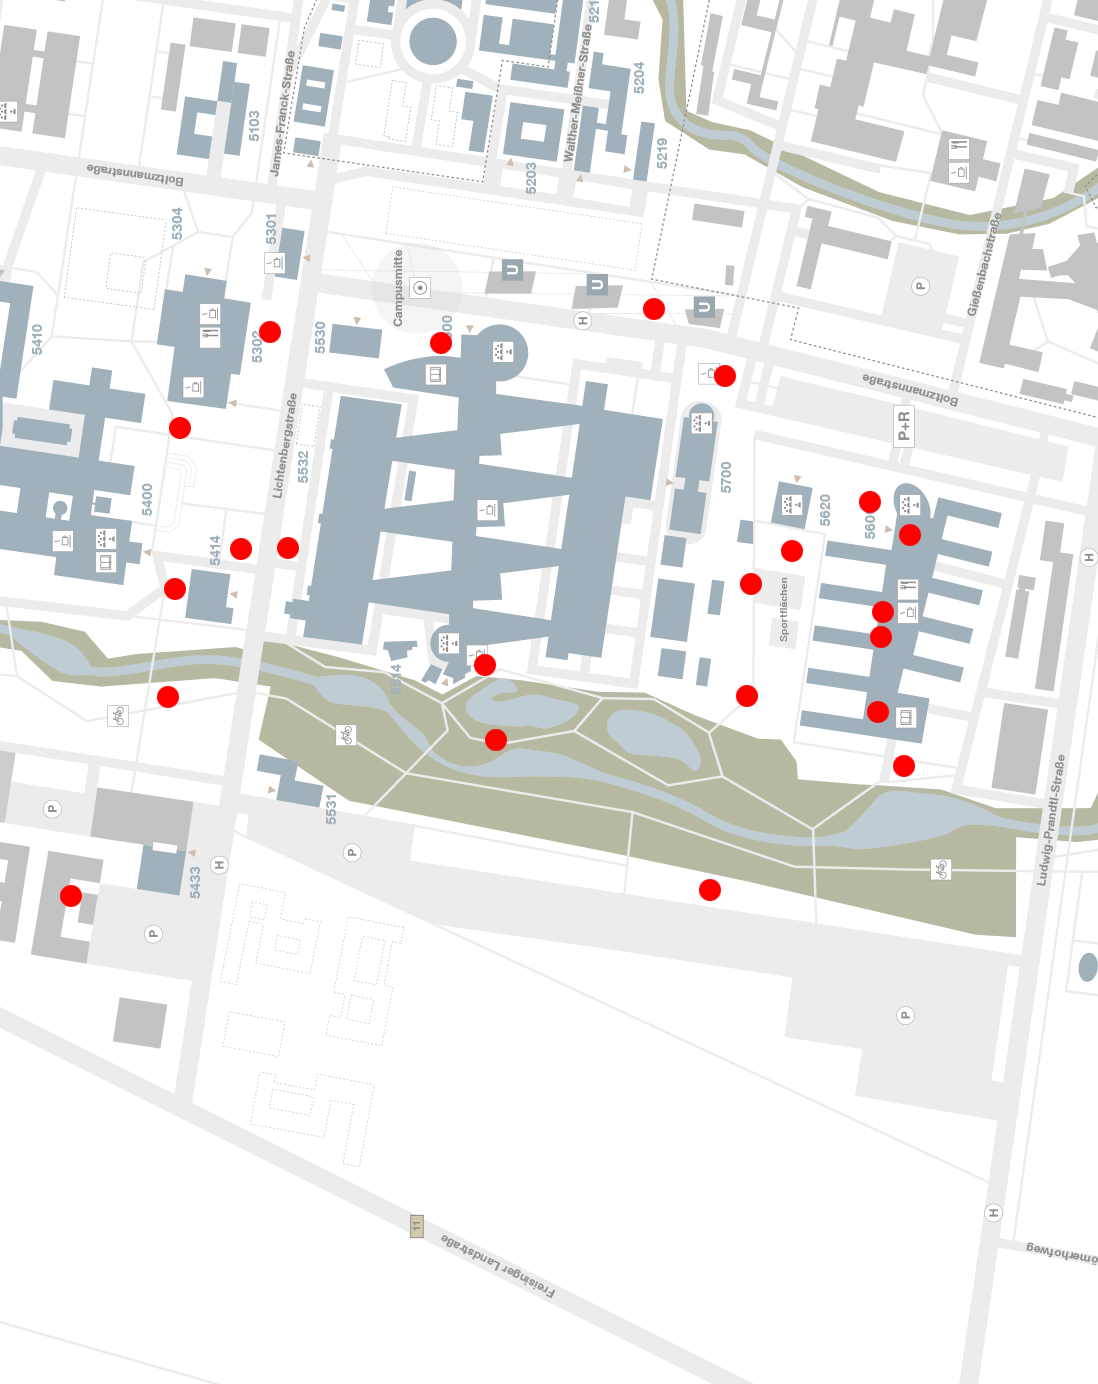
\includegraphics[width = \textwidth ]{Karte_neu_nur_punkte}
		\end{figure}
		\clearpage
	}

	
	
	
	
\end{document}
